%\documentclass[10pt,handout]{beamer}
\documentclass[10pt]{beamer}
\usepackage[english]{babel} % Anpassa efter svenska. Ger svensk logga.
\usepackage[utf8]{inputenc} % Anpassa efter linux
\usepackage{graphicx}
\usepackage{hyperref}
\usepackage{listings}
%\lstdefinelanguage{Stan}{
  morekeywords=[1]{functions,data,parameters,transformed,model,generated,quantities,%
    for,in,while,print,if,else,lower,upper,increment_log_prob,T,return,%
    reject,integrate_ode,integrate_ode_bdf,integrate_ode_rk45,target},%
  morekeywords=[2]{int,real,vector,%
    ordered,positive_ordered,simplex,unit_vector,%
    row_vector,matrix,%
    cholesky_factor_corr,cholesky_factor_cov,%
    coor_matrix,cov_matrix,%
    void},%
  morekeywords=[3]{%
    Phi,%
    Phi_approx,%
    abs,%
    acos,%
    acosh,%
    append_col,%
    append_row,%
    asin,%
    asinh,%
    atan,%
    atan2,%
    atanh,%
    bernoulli_cdf,%
    bernoulli_cdf_log,%
    bernoulli_lccdf,%
    bernoulli_lcdf,%
    bernoulli_logit_lpmf,%
    bernoulli_logit_lpmf,%
    bernoulli_lpmf,%
    bernoulli_lpmf,%
    bernoulli_rng,%
    bessel_first_kind,%
    bessel_second_kind,%
    beta_binomial_cdf,%
    beta_binomial_cdf_log,%
    beta_binomial_lccdf,%
    beta_binomial_lcdf,%
    beta_binomial_lpmf,%
    beta_binomial_lpmf,%
    beta_binomial_rng,%
    beta_cdf,%
    beta_cdf_log,%
    beta_lccdf,%
    beta_lcdf,%
    beta_lpdf,%
    beta_lpdf,%
    beta_rng,%
    binary_log_loss,%
    binomial_cdf,%
    binomial_cdf_log,%
    binomial_coefficient_log,%
    binomial_lccdf,%
    binomial_lcdf,%
    binomial_logit_lpmf,%
    binomial_logit_lpmf,%
    binomial_lpmf,%
    binomial_lpmf,%
    binomial_rng,%
    block,%
    categorical_logit_lpmf,%
    categorical_logit_lpmf,%
    categorical_lpmf,%
    categorical_lpmf,%
    categorical_rng,%
    cauchy_cdf,%
    cauchy_cdf_log,%
    cauchy_lccdf,%
    cauchy_lcdf,%
    cauchy_lpdf,%
    cauchy_lpdf,%
    cauchy_rng,%
    cbrt,%
    ceil,%
    chi_square_cdf,%
    chi_square_cdf_log,%
    chi_square_lccdf,%
    chi_square_lcdf,%
    chi_square_lpdf,%
    chi_square_lpdf,%
    chi_square_rng,%
    cholesky_decompose,%
    col,%
    cols,%
    columns_dot_product,%
    columns_dot_self,%
    cos,%
    cosh,%
    crossprod,%
    csr_extract_u,%
    csr_extract_v,%
    csr_extract_w,%
    csr_matrix_times_vector,%
    csr_to_dense_matrix,%
    cumulative_sum,%
    determinant,%
    diag_matrix,%
    diag_post_multiply,%
    diag_pre_multiply,%
    diagonal,%
    digamma,%
    dims,%
    dirichlet_lpdf,%
    dirichlet_lpdf,%
    dirichlet_rng,%
    distance,%
    dot_product,%
    dot_self,%
    double_exponential_cdf,%
    double_exponential_cdf_log,%
    double_exponential_lccdf,%
    double_exponential_lcdf,%
    double_exponential_lpdf,%
    double_exponential_lpdf,%
    double_exponential_rng,%
    e,%
    eigenvalues_sym,%
    eigenvectors_sym,%
    erf,%
    erfc,%
    exp,%
    exp2,%
    exp_mod_normal_cdf,%
    exp_mod_normal_cdf_log,%
    exp_mod_normal_lccdf,%
    exp_mod_normal_lcdf,%
    exp_mod_normal_lpdf,%
    exp_mod_normal_lpdf,%
    exp_mod_normal_rng,%
    expm1,%
    exponential_cdf,%
    exponential_cdf_log,%
    exponential_lccdf,%
    exponential_lcdf,%
    exponential_lpdf,%
    exponential_lpdf,%
    exponential_rng,%
    fabs,%
    falling_factorial,%
    fdim,%
    floor,%
    fma,%
    fmax,%
    fmin,%
    fmod,%
    frechet_cdf,%
    frechet_cdf_log,%
    frechet_lccdf,%
    frechet_lcdf,%
    frechet_lpdf,%
    frechet_lpdf,%
    frechet_rng,%
    gamma_cdf,%
    gamma_cdf_log,%
    gamma_lccdf,%
    gamma_lcdf,%
    gamma_lpdf,%
    gamma_lpdf,%
    gamma_p,%
    gamma_q,%
    gamma_rng,%
    gaussian_dlm_obs_lpdf,%
    gaussian_dlm_obs_lpdf,%
    get_lp,%
    gumbel_cdf,%
    gumbel_cdf_log,%
    gumbel_lccdf,%
    gumbel_lcdf,%
    gumbel_lpdf,%
    gumbel_lpdf,%
    gumbel_rng,%
    head,%
    hypergeometric_lpmf,%
    hypergeometric_lpmf,%
    hypergeometric_rng,%
    hypot,%
    if_else,%
    inc_beta,%
    int_step,%
    inv,%
    inv_chi_square_cdf,%
    inv_chi_square_cdf_log,%
    inv_chi_square_lccdf,%
    inv_chi_square_lcdf,%
    inv_chi_square_lpdf,%
    inv_chi_square_lpdf,%
    inv_chi_square_rng,%
    inv_cloglog,%
    inv_gamma_cdf,%
    inv_gamma_cdf_log,%
    inv_gamma_lccdf,%
    inv_gamma_lcdf,%
    inv_gamma_lpdf,%
    inv_gamma_lpdf,%
    inv_gamma_rng,%
    inv_logit,%
    inv_phi,%
    inv_sqrt,%
    inv_square,%
    inv_wishart_lpdf,%
    inv_wishart_lpdf,%
    inv_wishart_rng,%
    inverse,%
    inverse_spd,%
    is_inf,%
    is_nan,%
    lbeta,%
    lchoose,%
    lgamma,%
    lkj_corr_cholesky_lpdf,%
    lkj_corr_cholesky_lpdf,%
    lkj_corr_cholesky_rng,%
    lkj_corr_lpdf,%
    lkj_corr_lpdf,%
    lkj_corr_rng,%
    lmgamma,%
    lmultiply,%
    log,%
    log10,%
    log1m,%
    log1m_exp,%
    log1m_inv_logit,%
    log1p,%
    log1p_exp,%
    log2,%
    log_determinant,%
    log_diff_exp,%
    log_falling_factorial,%
    log_inv_logit,%
    log_mix,%
    log_rising_factorial,%
    log_softmax,%
    log_sum_exp,%
    logistic_cdf,%
    logistic_cdf_log,%
    logistic_lccdf,%
    logistic_lcdf,%
    logistic_lpdf,%
    logistic_lpdf,%
    logistic_rng,%
    logit,%
    lognormal_cdf,%
    lognormal_cdf_log,%
    lognormal_lccdf,%
    lognormal_lcdf,%
    lognormal_lpdf,%
    lognormal_lpdf,%
    lognormal_rng,%
    machine_precision,%
    max,%
    mdivide_left_tri_low,%
    mdivide_right_tri_low,%
    mean,%
    min,%
    modified_bessel_first_kind,%
    modified_bessel_second_kind,%
    multi_gp_cholesky_lpdf,%
    multi_gp_cholesky_lpdf,%
    multi_gp_lpdf,%
    multi_gp_lpdf,%
    multi_normal_cholesky_lpdf,%
    multi_normal_cholesky_lpdf,%
    multi_normal_cholesky_rng,%
    multi_normal_lpdf,%
    multi_normal_lpdf,%
    multi_normal_prec_lpdf,%
    multi_normal_prec_lpdf,%
    multi_normal_rng,%
    multi_student_t_lpdf,%
    multi_student_t_lpdf,%
    multi_student_t_rng,%
    multinomial_lpmf,%
    multinomial_lpmf,%
    multinomial_rng,%
    multiply_log,%
    multiply_lower_tri_self_transpose,%
    neg_binomial_2_cdf,%
    neg_binomial_2_cdf_log,%
    neg_binomial_2_lccdf,%
    neg_binomial_2_lcdf,%
    neg_binomial_2_log_lpmf,%
    neg_binomial_2_log_lpmf,%
    neg_binomial_2_log_rng,%
    neg_binomial_2_lpmf,%
    neg_binomial_2_lpmf,%
    neg_binomial_2_rng,%
    neg_binomial_cdf,%
    neg_binomial_cdf_log,%
    neg_binomial_lccdf,%
    neg_binomial_lcdf,%
    neg_binomial_lpmf,%
    neg_binomial_lpmf,%
    neg_binomial_rng,%
    negative_infinity,%
    normal_cdf,%
    normal_cdf_log,%
    normal_lccdf,%
    normal_lcdf,%
    normal_lpdf,%
    normal_lpdf,%
    normal_rng,%
    not_a_number,%
    num_elements,%
    ordered_logistic_lpmf,%
    ordered_logistic_lpmf,%
    ordered_logistic_rng,%
    owens_t,%
    pareto_cdf,%
    pareto_cdf_log,%
    pareto_lccdf,%
    pareto_lcdf,%
    pareto_lpdf,%
    pareto_lpdf,%
    pareto_rng,%
    pareto_type_2_cdf,%
    pareto_type_2_cdf_log,%
    pareto_type_2_lccdf,%
    pareto_type_2_lcdf,%
    pareto_type_2_lpdf,%
    pareto_type_2_lpdf,%
    pareto_type_2_rng,%
    pi,%
    poisson_cdf,%
    poisson_cdf_log,%
    poisson_lccdf,%
    poisson_lcdf,%
    poisson_log_lpmf,%
    poisson_log_lpmf,%
    poisson_log_rng,%
    poisson_lpmf,%
    poisson_lpmf,%
    poisson_rng,%
    positive_infinity,%
    pow,%
    prod,%
    qr_Q,%
    qr_R,%
    quad_form,%
    quad_form_diag,%
    quad_form_sym,%
    rank,%
    rayleigh_cdf,%
    rayleigh_cdf_log,%
    rayleigh_lccdf,%
    rayleigh_lcdf,%
    rayleigh_lpdf,%
    rayleigh_lpdf,%
    rayleigh_rng,%
    rep_array,%
    rep_matrix,%
    rep_row_vector,%
    rep_vector,%
    rising_factorial,%
    round,%
    row,%
    rows,%
    rows_dot_product,%
    rows_dot_self,%
    scaled_inv_chi_square_cdf,%
    scaled_inv_chi_square_cdf_log,%
    scaled_inv_chi_square_lccdf,%
    scaled_inv_chi_square_lcdf,%
    scaled_inv_chi_square_lpdf,%
    scaled_inv_chi_square_lpdf,%
    scaled_inv_chi_square_rng,%
    sd,%
    segment,%
    sin,%
    singular_values,%
    sinh,%
    size,%
    skew_normal_cdf,%
    skew_normal_cdf_log,%
    skew_normal_lccdf,%
    skew_normal_lcdf,%
    skew_normal_lpdf,%
    skew_normal_lpdf,%
    skew_normal_rng,%
    softmax,%
    sort_asc,%
    sort_desc,%
    sort_indices_asc,%
    sort_indices_desc,%
    sqrt,%
    sqrt2,%
    square,%
    squared_distance,%
    step,%
    student_t_cdf,%
    student_t_cdf_log,%
    student_t_lccdf,%
    student_t_lcdf,%
    student_t_lpdf,%
    student_t_lpdf,%
    student_t_rng,%
    sub_col,%
    sub_row,%
    sum,%
    tail,%
    tan,%
    tanh,%
    tcrossprod,%
    tgamma,%
    to_array_1d,%
    to_array_2d,%
    to_matrix,%
    to_row_vector,%
    to_vector,%
    trace,%
    trace_gen_quad_form,%
    trace_quad_form,%
    trigamma,%
    trunc,%
    uniform_cdf,%
    uniform_cdf_log,%
    uniform_lccdf,%
    uniform_lcdf,%
    uniform_lpdf,%
    uniform_lpdf,%
    uniform_rng,%
    variance,%
    von_mises_lpdf,%
    von_mises_lpdf,%
    von_mises_rng,%
    weibull_cdf,%
    weibull_cdf_log,%
    weibull_lccdf,%
    weibull_lcdf,%
    weibull_lpdf,%
    weibull_lpdf,%
    weibull_rng,%
    wiener_lpdf,%
    wiener_lpdf,%
    wishart_lpdf,%
    wishart_lpdf,%
    wishart_rng
  },%
  otherkeywords={<-,~,+=,=},%
  sensitive=true,%
  morecomment=[l]{\#},%
  morecomment=[l]{//},%
  morecomment=[n]{/*}{*/},%
  string=[d]"%,
  literate={<-}{{$\leftarrow$}}1 {~}{{$\sim$}}1%
}
 % Stan listing
\usepackage{lstbayes}
\usepackage[all,poly,ps,color]{xy}


\hypersetup{
    colorlinks=true,
    linkcolor=blue,
    filecolor=magenta,
    urlcolor=cyan,
}
\usepackage{../common/beamerthemeUppsala}
%\usetheme{Uppsala}
%\usecolortheme{UU} % Anpassa efter UU:s frger och logga
%\hypersetup{pdfpagemode=FullScreen} % Adobe Reader ska ppna fullskrm
\setbeamertemplate{itemize items}[circle]

% \usepackage{beamerthemesplit}
\usepackage{amsmath,amsfonts,amssymb}
% \usepackage{amssymb}
% \usepackage{graphics}
% \usepackage{graphicx}
% \usepackage{epsfig}
% \usepackage[latin1]{inputenc}
 \usepackage{color}
% \usepackage{fancybox}
% \usepackage{psfrag}
% \usepackage[english]{babel}
 \setbeamertemplate{footline}{\hfill\insertframenumber/\inserttotalframenumber}

% Input new commands
%\usepackage{bm}
%\usepackage{natbib}
\newcommand{\bfm}[1]   {\mbox{\boldmath{${#1}$}}}
\newcommand{\Prob}   {\mbox{\textnormal{P}}}
\def\eqd{\,{\buildrel d \over =}\,}

% Vector/Matrix definitions (in bold type)
\newcommand{\vect}[1]{\mathbf{#1}}
\newcommand{\vectb}[1]{\bm{#1}}

% Differential operator 'd' as upright as in (use \dd)
\newcommand{\dd}{\; \mathrm{d}}

% Gaussian normal distribution (use \N)
\newcommand{\N}{\mathcal{N}} %% or \mathrm{N}

% Uniform distribution (use \Uni or \U)
\newcommand{\Uni}{\mathcal{U}} %% or \mathrm{U}
\newcommand{\U}{\mathcal{U}} %% or \mathrm{U}

% Matrix transpose (use \T)
\newcommand{\T}{^{\mathsf{T}}}

% Blockdiagonal matrices (use \blockdiag)
\newcommand{\blockdiag}{\mathrm{blockdiag}}

% Define inner product '<f,g>' notation (use \innerp{#1})
\providecommand{\innerp}[1]{\left\langle#1\right\rangle}

\def\o{{\mathbf o}}
\def\t{{\mathbf \theta}}
\def\w{{\mathbf w}}
\def\x{{\mathbf x}}
\def\y{{\mathbf y}}
\def\z{{\mathbf z}}



% Other math symbols and notation
\newcommand{\D}{^\mathsf{\dagger}}
\newcommand{\R}{\mathbb{R}}
\newcommand{\erf}{\mathrm{erf}}
\newcommand{\E}{\mathrm{E}}
\newcommand{\var}{\mathrm{var}}
\newcommand{\Var}{\mathrm{Var}}
\newcommand{\cov}{\mathrm{cov}}
\newcommand{\Ker}{\operatorname{Ker}}
\newcommand{\Ran}{\operatorname{Ran}}
\providecommand{\norm}[1]{\lVert#1\rVert}
\providecommand{\op}[1]{\mathcal{#1}}
\newcommand{\arccot}{\mathrm{arccot}}
\providecommand{\Hspace}[1]{\mathscr{#1}}
\providecommand{\fourier}[1]{\mathscr{#1}}

\newcommand{\kin}{k^{\rm in}}
\newcommand{\kout}{k^{\rm out}}
\newcommand{\gi}{{R_0}}
\newcommand{\eff}{{E_{\rm max}}}
\newcommand{\ESS}{\mathrm{ESS}}
\newcommand{\HN}{{\rm N^+}}
\newcommand{\lN}{{\rm LN}}

\DeclareMathOperator{\Sd}{Sd}
\DeclareMathOperator{\sd}{sd}
\DeclareMathOperator{\Gammad}{Gamma}
\DeclareMathOperator{\Invgamma}{Inv-gamma}
\DeclareMathOperator{\Bin}{Bin}
\DeclareMathOperator{\Negbin}{Neg-bin}
\DeclareMathOperator{\Poisson}{Poisson}
\DeclareMathOperator{\Beta}{Beta}
\DeclareMathOperator{\logit}{logit}
\DeclareMathOperator{\BF}{BF}
\DeclareMathOperator{\Invchi2}{Inv-\chi^2}
\DeclareMathOperator{\NInvchi2}{N-Inv-\chi^2}
\DeclareMathOperator{\InvWishart}{Inv-Wishart}
\DeclareMathOperator{\tr}{tr}
% \DeclareMathOperator{\Pr}{Pr}
\def\euro{{\footnotesize \EUR\, }}
\DeclareMathOperator{\rep}{\mathrm{rep}}


\def\dashxy(#1){%
  /xydash{[#1] 0 setdash}def}
\def\grayxy(#1){%
  /xycolor{#1 setgray}def}
\newgraphescape{D}[1]{!{\ar @*{[!\dashxy(2 2)]} "#1"}}
\newgraphescape{P}[1]{!{\ar "#1"}}
\newgraphescape{F}[1]{!{*+=<2em>[F=]{#1}="#1"}}
\newgraphescape{O}[1]{!{*+=<2em>[F]{#1}="#1"}}
\newgraphescape{V}[1]{!{*+=<2em>[o][F]{#1}="#1"}}
\newgraphescape{B}[3]{!{{ "#1"*+#3\frm{} }.{ "#2"*+#3\frm{} } *+[F:!\grayxy(0.75)]\frm{}}}

%%%%%%%%%%%%%%%%%%%%%%%%%%%%%%%%%%%%%%%%%%%%%%%%%%%%%%%%%%%%%%%%%%

\setlength{\parskip}{3mm}
\title[]{{\color{black}Bayesian Statistics and Data Analysis \\ Lecture 8a}}
\author[]{M{\aa}ns Magnusson \\ Department of Statistics, Uppsala University \\ Thanks to Aki Vehtari, Aalto University}
\date{}

\begin{document}

\frame{\titlepage
% \thispagestyle{empty}
}

%%%%%%%%%%%%%%%%%%%%%%%%%%%%%%%%%%%%%%%%%%%%%%%%%%%%%%%%%%%%%%%%%%


\section{Model Checking and Assessment}
\frame{\sectionpage}



\begin{frame}{The Box process: Probabilistic modeling}

\begin{figure}
    \centering
    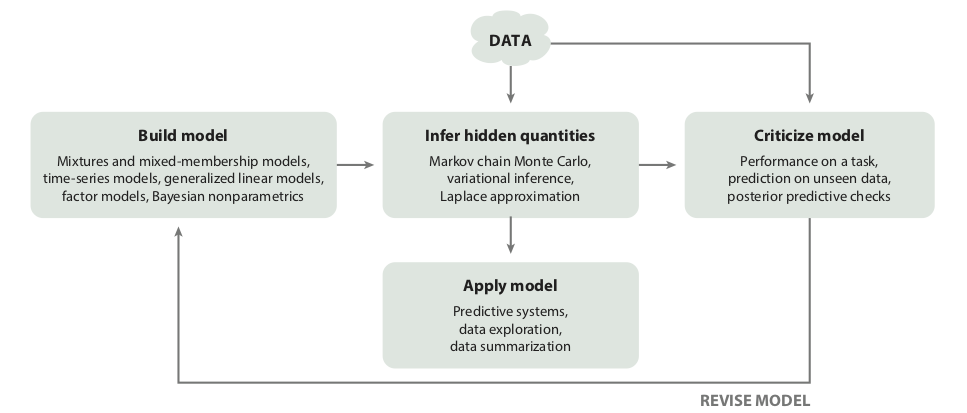
\includegraphics[width=1\textwidth]{figs/Boxs_loop.png}
    \caption{The Box approach (Box, 1976, Blei, 2014)}
\end{figure}
\end{frame}

\begin{frame}

\frametitle{Model assessment}

  \begin{itemize}
  \item<+-> Sensibility with respect to additional information not used in model
    \begin{itemize}
    \item e.g., if posterior would claim that hazardous chemical
      decreases probability of death
    \end{itemize}
  \item<+-> External validation
    \begin{itemize}
    \item compare predictions to completely new observations
%    \item cf. relativity theory predictions
    \end{itemize}
  \item<+-> Internal validation
    \begin{itemize}
    \item posterior predictive checking
    \item cross-validation predictive checking
    \end{itemize}
  \end{itemize}

\end{frame}

\section{Posterior predictive checking}
\frame{\sectionpage}

\begin{frame}[fragile]
\frametitle{Posterior predictive checking -- example}

  \begin{itemize}
  \item<1-> Newcombs speed of light measurements
    \begin{itemize}
    \item model $y \sim \N(\mu,\sigma)$ with prior $(\mu, \log \sigma) \propto 1$
    \end{itemize}
  \item<2-> Posterior predictive replicate $y^{\rm rep}$
    \begin{itemize}
    \item<3-> draw $\mu^{(s)},\sigma^{(s)}$ from the posterior $p(\mu,\sigma|y)$
    \item<4-> draw $y^{\mathrm{rep}\,(s)}$ from $\N(\mu^{(s)},\sigma^{(s)})$
    \item<5-> repeat $n$ times to get $y^{\mathrm{rep}}$ with $n$ replicates\\~\\
    \uncover<6->{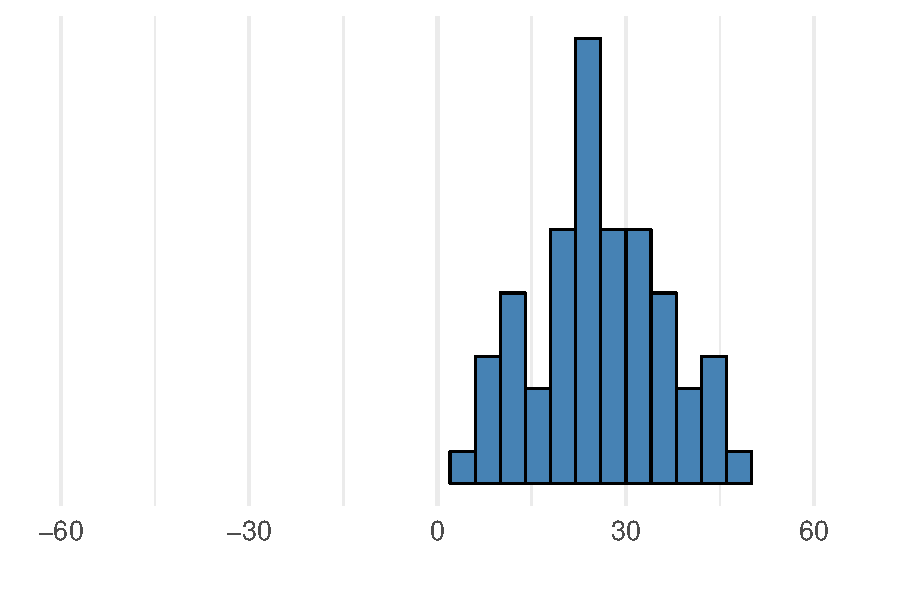
\includegraphics[width=7cm]{figs/light_ppc_1hist.pdf}}
      \end{itemize}
    \end{itemize}

\end{frame}


\begin{frame}

\frametitle{Replicates vs. future observation}

  \begin{itemize}
  \item Predictive $\tilde{y}$ is the next not yet observed possible
    observation. \pause
    % TODO: Add predictive distribution here
    \item $y^{\mathrm{rep}}$ refers to replicating the \uured{whole
    experiment} (potentially with same values of $x$)\\i.e. obtaining as
    many replicated observations as in the original data.
    % TODO: Double check that y^rep is also a predictive distribution
  \end{itemize}

\end{frame}


\begin{frame}[fragile]

\frametitle{Posterior predictive checking -- example}

  \begin{itemize}
  \item<1-> Generate replicated datasets $y^{\rm rep}$
  %\item<2-> Commonly done using Monte Carlo draws
  % TODO: Double check how yrep is draw (ie using monte carlo draws)
  \item<2-> Compare to the original dataset
  \end{itemize}
  \vspace{-1\baselineskip}
  \uncover<3->{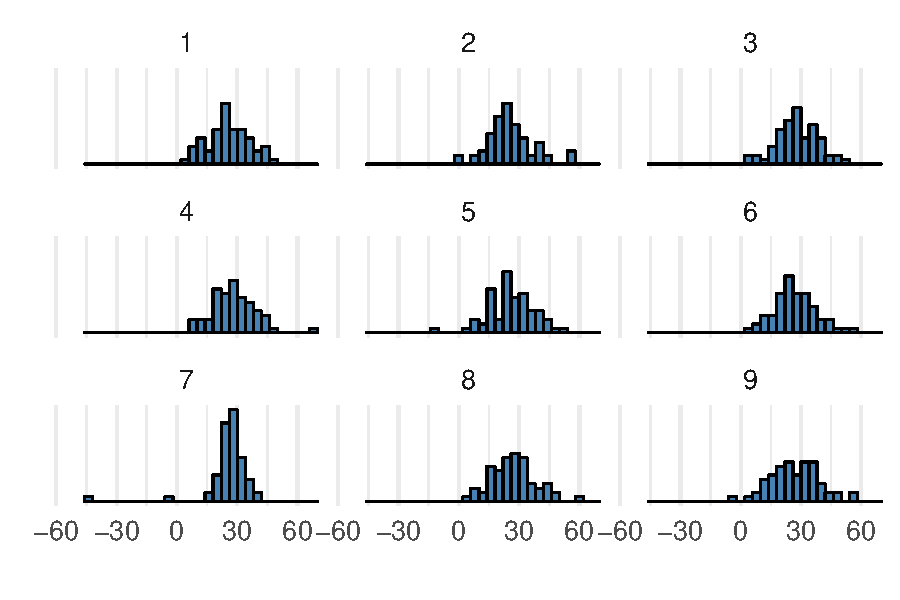
\includegraphics[width=9cm]{figs/light_ppc_10hist.pdf}}

\end{frame}


\begin{frame}

\frametitle{Posterior predictive checking with test statistic}

  \begin{itemize}
  \item Replicated data sets $y^{\rep}$
  \item Test quantity (or discrepancy measure) $T(y,\theta)$
    \begin{itemize}
    \item summary quantity for the observed data $T(y,\theta)$
    \item summary quantity for a replicated data $T(y^{\rep},\theta)$
    \item can be easier to compare summary quantities ($y^{\rep}$ statistics) than data sets
    \end{itemize}
  \end{itemize}

\end{frame}

% TODO: Define test statistic here from the book.

\begin{frame}[fragile]

\frametitle{Posterior predictive checking -- example}

  \begin{itemize}
  \item<1-> Compute test statistic for data $T(y,\theta)=\min(y)$
  \item<2-> Compute test statistic $\min(y^{\rm rep})$ for many replicated datasets
  \end{itemize}
  \vspace{-1.5\baselineskip}
  \uncover<3->{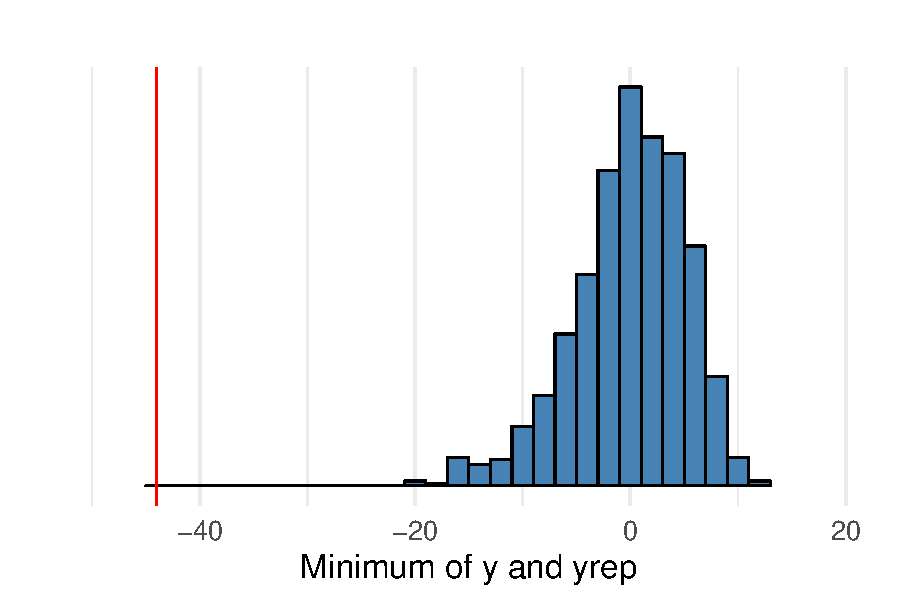
\includegraphics[width=9cm]{figs/light_ppc_min.pdf}}

\end{frame}


\begin{frame}[fragile]

\frametitle{Posterior predictive checking -- example}

  \begin{itemize}
  \item<1-> Good test statistic is \href{https://en.wikipedia.org/wiki/Ancillary_statistic}{ancillary} (or almost)
    \begin{itemize}
    \item a statistic $T(X)$ that does not depend on the parameters of the model are ancillary\\e.g. in a normal model with \uured{known} $\sigma^2$,
    \[
    s^2 = \sum_i^n \frac{(x_i-\bar{x})^2}{n-1}\,,
    \]
    is ancillary ($\mu$ cancel out).
    \end{itemize}
  \item<2-> Bad test statistic is highly dependent of the parameters
    \begin{itemize}
    \item e.g. variance (or mean) for normal model with \uured{unknown} $\sigma^2$. If $\sigma^2$ changes so will $T(X)$.
    \end{itemize}
  \item<3-> We want to \uured{identify problems} in data not captured by the \uured{model}
  \end{itemize}

\end{frame}

\begin{frame}[fragile]

\frametitle{Posterior predictive checking -- example}

  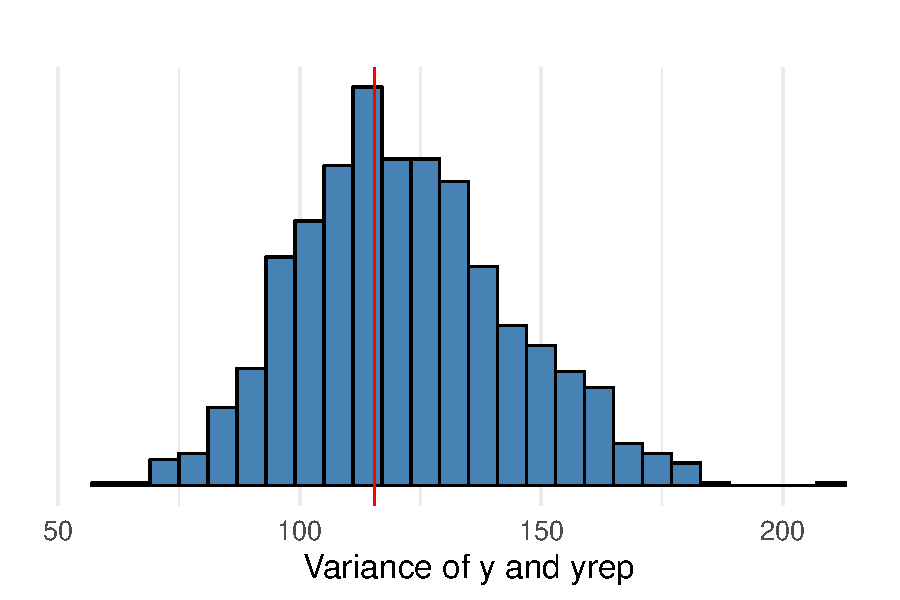
\includegraphics[width=9cm]{figs/light_ppc_var.pdf}

\end{frame}


\begin{frame}[fragile]

\frametitle{Posterior predictive $p$-value}

  \begin{itemize}
  \item<1-> \textit{Posterior predictive $p$-value}
    \begin{eqnarray*}
      p & = & \Pr(T(y^{\rep},\theta)\geq T(y,\theta)|y)\\
      & = & \int\int
      I_{T(y^{\rep},\theta)\geq T(y,\theta)}p(y^{\rep}|\theta)p(\theta|y)dy^{\rep}d\theta
    \end{eqnarray*}
    where $I$ is an indicator function
    \begin{itemize}
    \item<2-> having $(y^{\rep\,(s)},\theta^{(s)})$ from the posterior predictive
      distribution (Monte Carlo):
      \begin{equation*}
        T(y^{\rep (s)},\theta^{(s)})\geq T(y,\theta^{(s)}), \quad s=1,\ldots,S
      \end{equation*}
    \end{itemize}
    \vspace{-1.5\baselineskip}
  \item<3-> Posterior predictive $p$-value (ppp-value):\\
    \uured{could difference between the model and data  arise by chance}
  \item<4-> Not commonly used, since the distribution of test
    statistic $T(y,\theta)$ has more information
  \end{itemize}

\end{frame}

% TODOD: Add the special case when thtea is know then, p values follows a uniform distributions. See book.

\begin{frame}[fragile]

\frametitle{Marginal and CV predictive checking}

  \begin{itemize}
  \item Consider marginal predictive distributions $p(\tilde{y}_i|y)$
    and each observation separately
    \begin{itemize}
    \item marginal posterior p-values
      \begin{align*}
        p_i = \mbox{Pr}(T(y_i^{\rep}) \leq T(y_i) | y)
      \end{align*}
      if $T(y_i)=y_i$
      \begin{align*}
        p_i = \mbox{Pr}(y_i^{\rep} \leq y_i | y)
      \end{align*}
    \end{itemize}
  \item<2-> if $Pr(\tilde{y}_i|y)$ well calibrated, distribution of $p_i$
    would be uniform between 0 and 1
    \begin{itemize}
    \item holds better for cross-validation predictive tests: $Pr(\tilde{y}_i|y_{-i})$
      (cross-validation)
    \end{itemize}
  \end{itemize}

\end{frame}

\begin{frame}[fragile]

\frametitle{Marginal predictive checking - Example}

  \begin{itemize}
  \item Marginal tail area or Probability integral transform (PIT)
    \begin{align*}
      p_i = p(y_i^{\rep} \leq y_i | y)
    \end{align*}
  \item if $p(\tilde{y}_i|y)$ is well calibrated, distribution of $p_i$'s
    would be uniform between 0 and 1
  \end{itemize}
  \vspace{-1.5\baselineskip}
  \uncover<2->{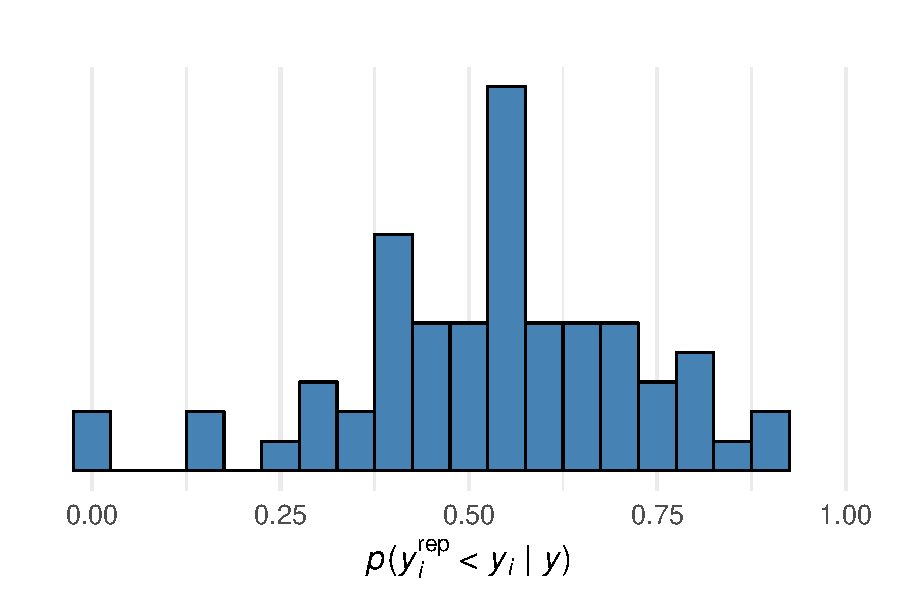
\includegraphics[width=9cm]{figs/light_ppc_pit.pdf}}

\end{frame}


\begin{frame}

\frametitle{Sensitivity analysis}

  \begin{itemize}
  \item How much different choices in model structure and priors affect the results
    \begin{itemize}
      \item<2-> test different models and priors
      \item<3-> alternatively combine different models to one model
        \begin{itemize}
        \item e.g. hierarchical model instead of separate and pooled
        \item e.g. $t$ distribution contains Gaussian as a special case
      \end{itemize}
      \item<3-> robust models are good for testing sensitivity to ``outliers''
        \begin{itemize}
        \item e.g. $t$ instead of Gaussian
        \end{itemize}
    \end{itemize}
    \item<4-> Compare sensitivity of essential inference quantities
      \begin{itemize}
      \item extreme quantiles are more sensitive than means and medians
      \item extrapolation is more sensitive than interpolation
      \end{itemize}
    \end{itemize}

\end{frame}

\begin{frame}

\frametitle{Example: Exposure to air pollution}

  \begin{itemize}
  \item Example from Jonah Gabry, Daniel Simpson, Aki Vehtari, Michael
    Betancourt, and Andrew Gelman (2019). Visualization in Bayesian
    workflow. \url{https://doi.org/10.1111/rssa.12378}
  \item Estimation of human exposure to air pollution from particulate
    matter measuring less than 2.5 microns in diameter ($\mathrm{PM}_{2.5}$)
    \begin{itemize}
    \item Exposure to $\mathrm{PM}_{2.5}$ is linked to a number of
      poor health outcomes and a recent report estimated that
      $\mathrm{PM}_{2.5}$ is responsible for three million deaths
      worldwide each year (Shaddick et al., 2017)
    \item In order to estimate the public health effect of ambient
      $\mathrm{PM}_{2.5}$, we need a good estimate of the
      $\mathrm{PM}_{2.5}$ concentration at the same spatial resolution
      as our population estimates.
    \end{itemize}
\end{itemize}

\end{frame}

\begin{frame}

\frametitle{Example: Exposure to air pollution}

  \begin{itemize}
  \item Direct measurements of PM 2.5 from ground monitors at 2980
    locations
  \item High-resolution satellite data of aerosol optical depth
  \end{itemize}
  \begin{center}
    \only<1>{\vspace{-1.8\baselineskip}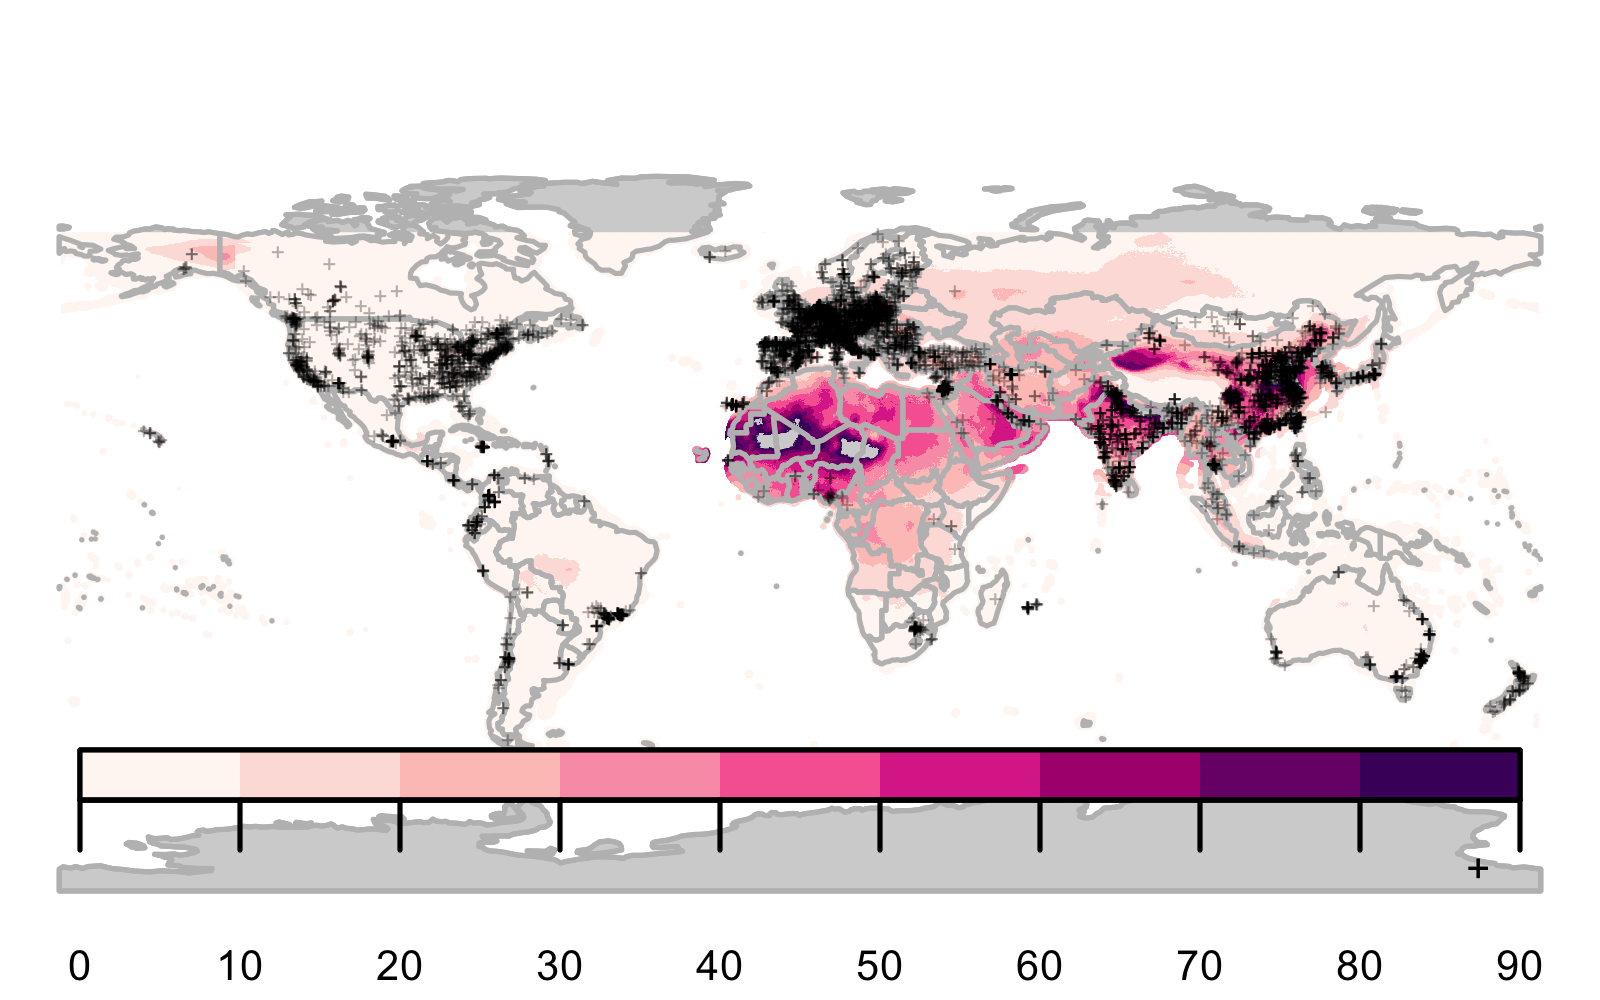
\includegraphics[height=6cm]{figs/map-data.png}}
    \only<2>{\vspace{-1.8\baselineskip}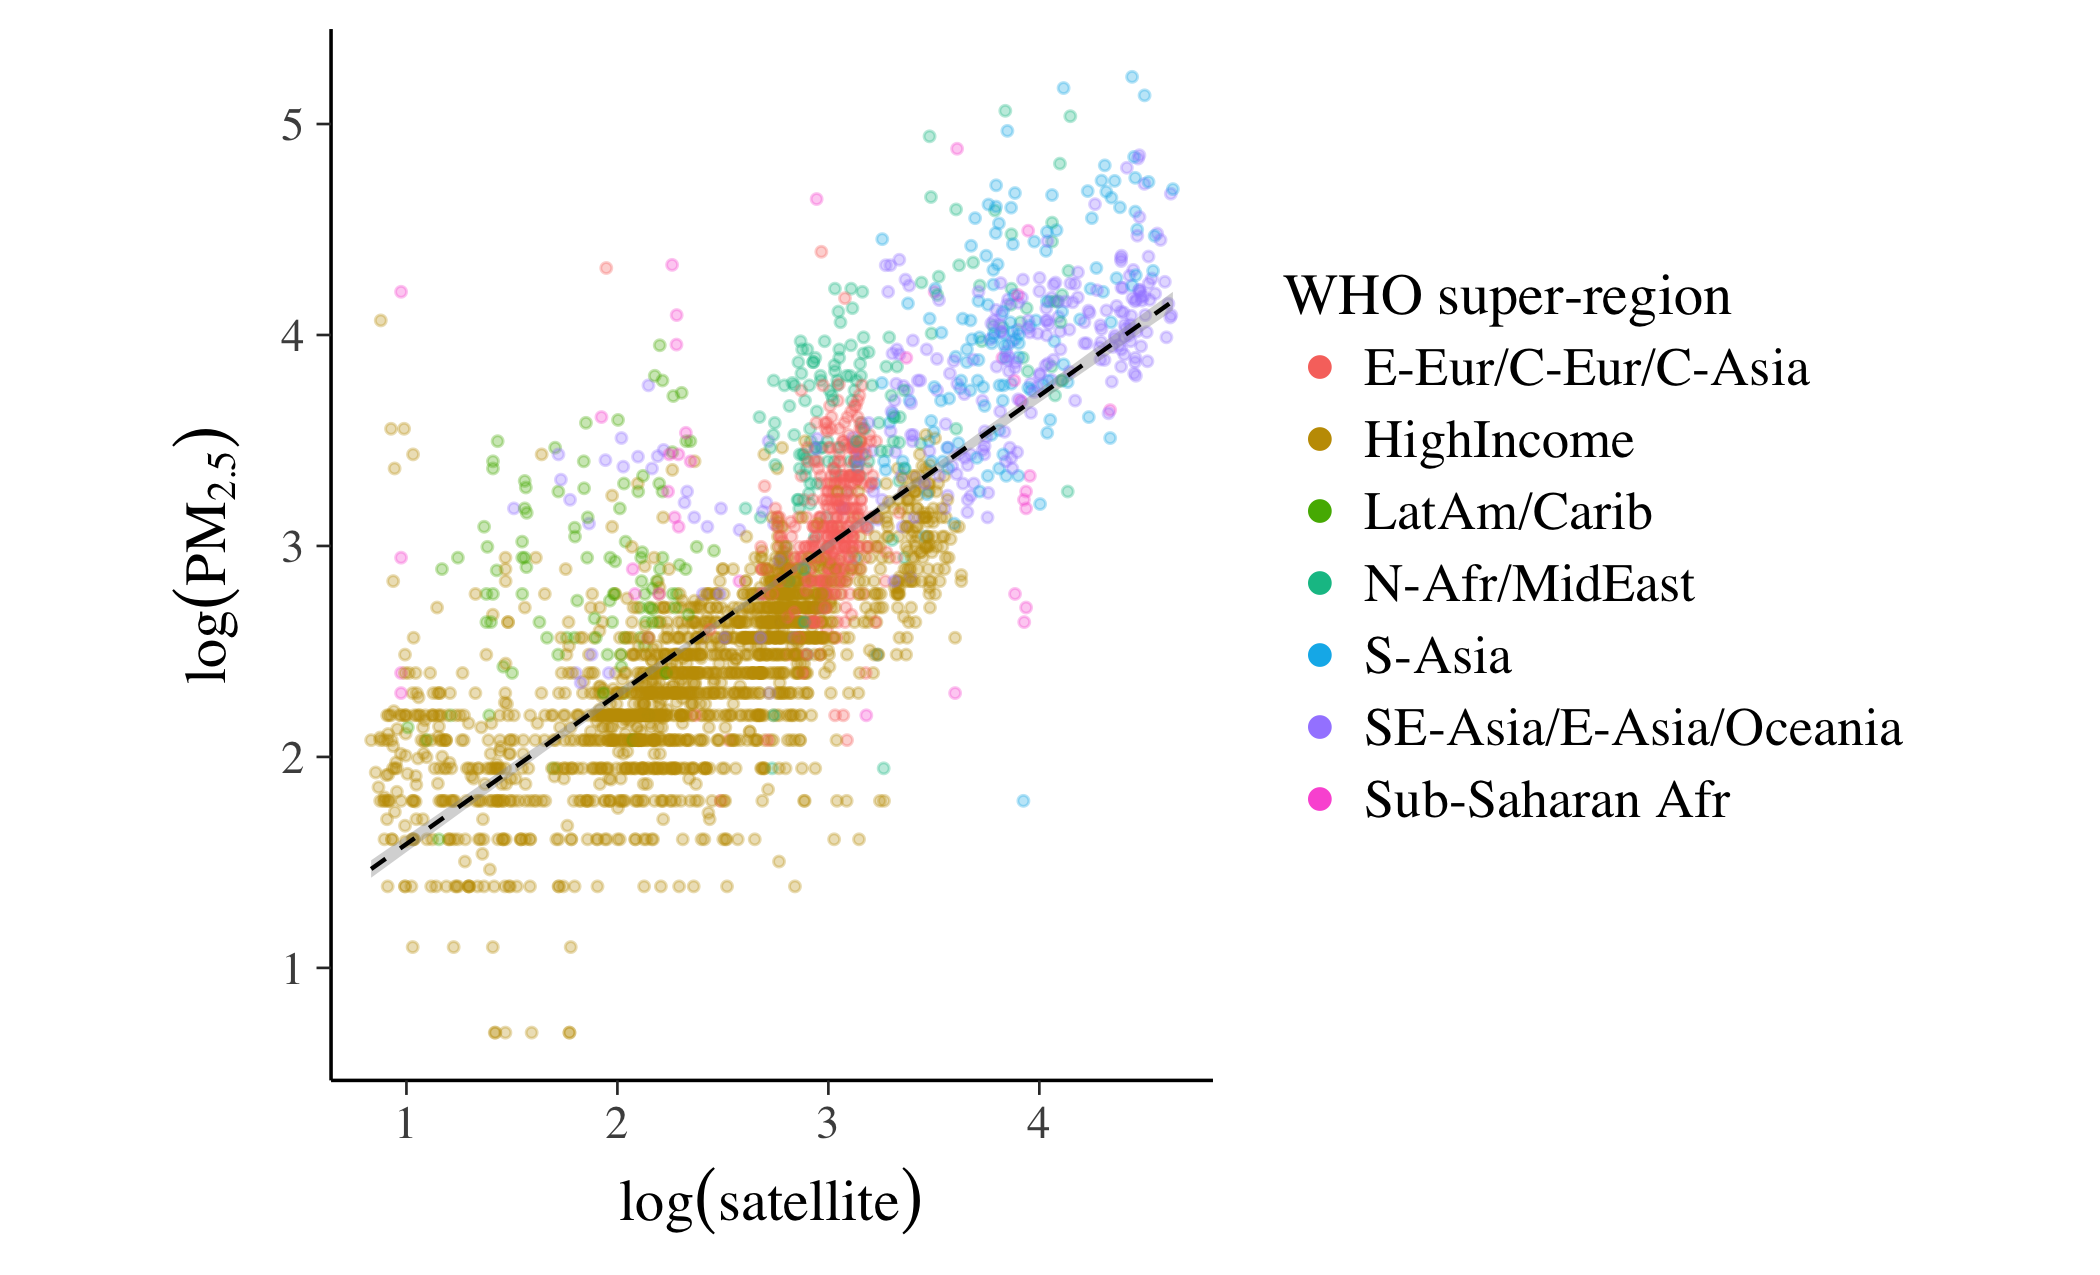
\includegraphics[height=6cm]{figs/plot1.png}}
    \only<3>{\hspace{-3cm}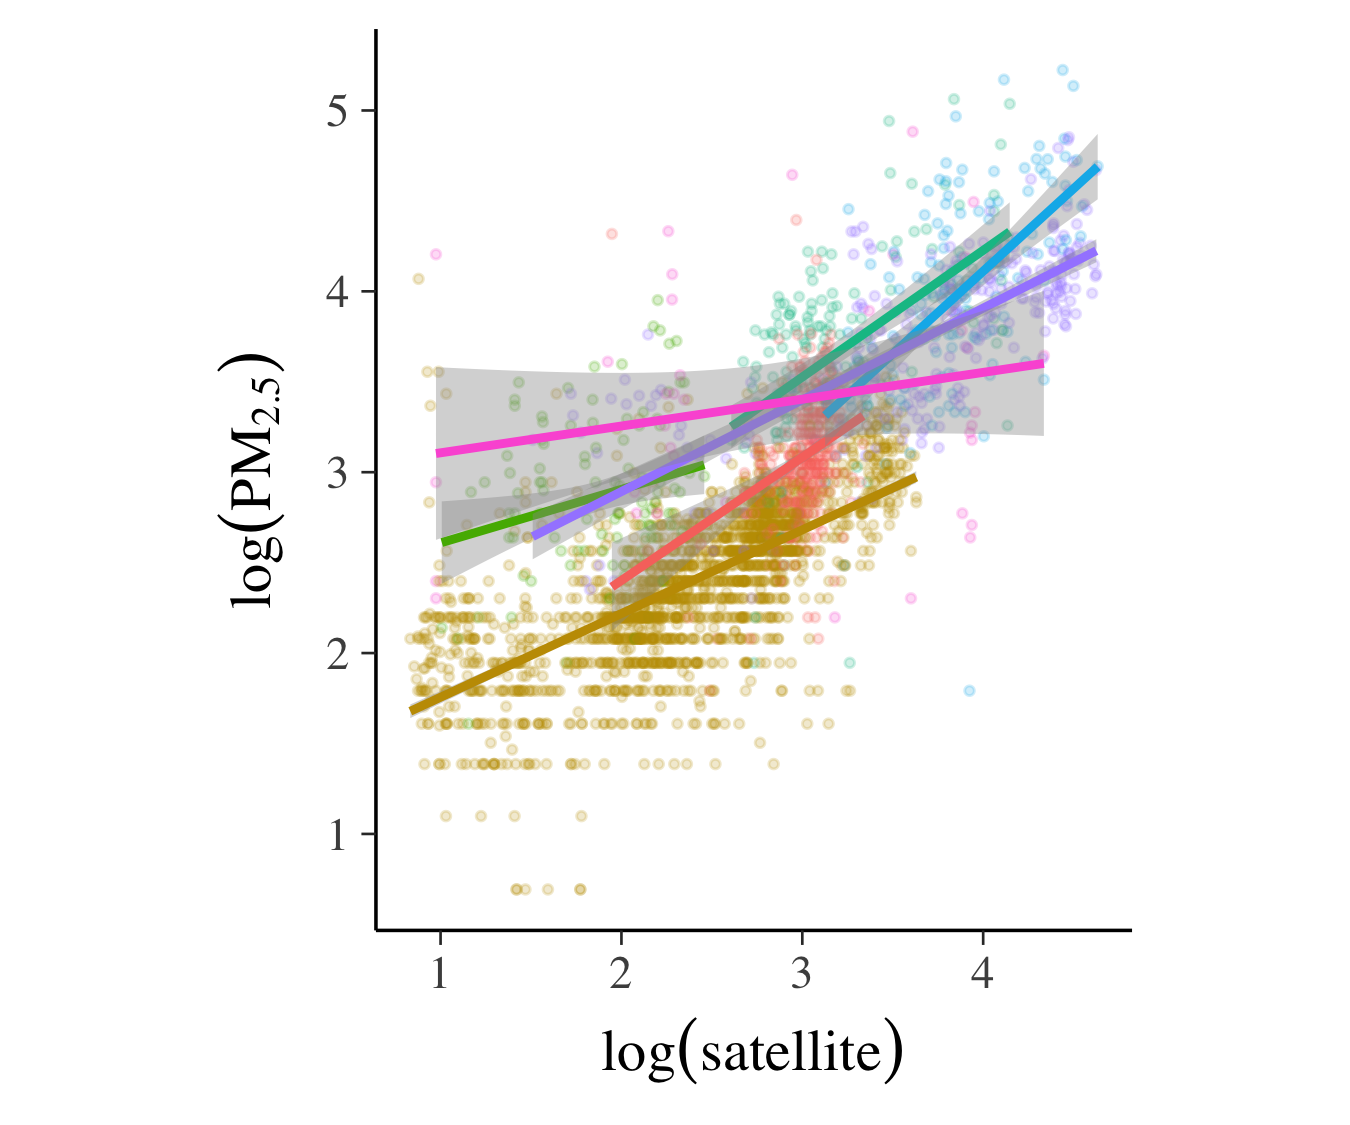
\includegraphics[height=5.55cm]{figs/plot2.png}}
\end{center}
\end{frame}


\begin{frame}

\frametitle{Example: Prior predictive checking}

  \begin{center}
    \only<1>{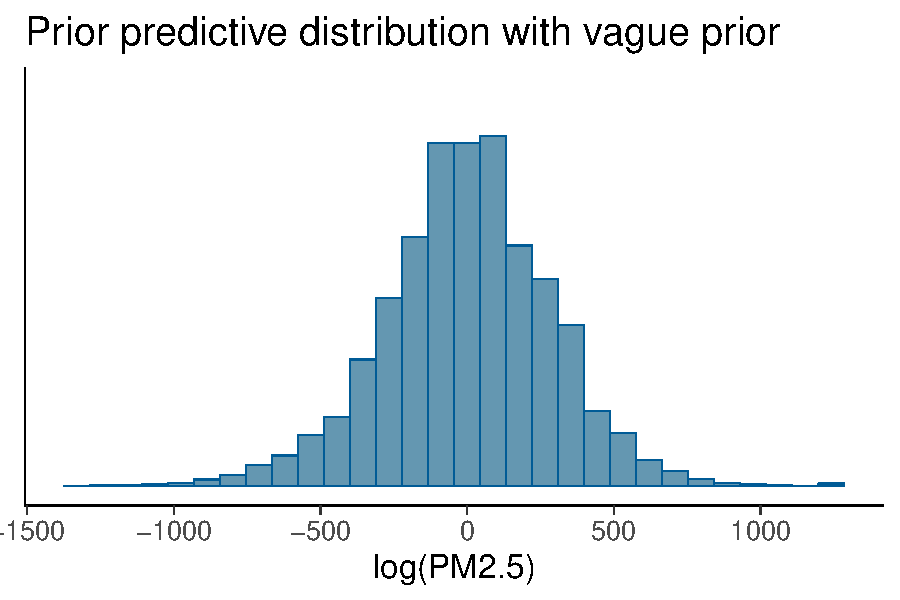
\includegraphics[width=8cm]{figs/pm25_pp1a.pdf}}
    \only<2>{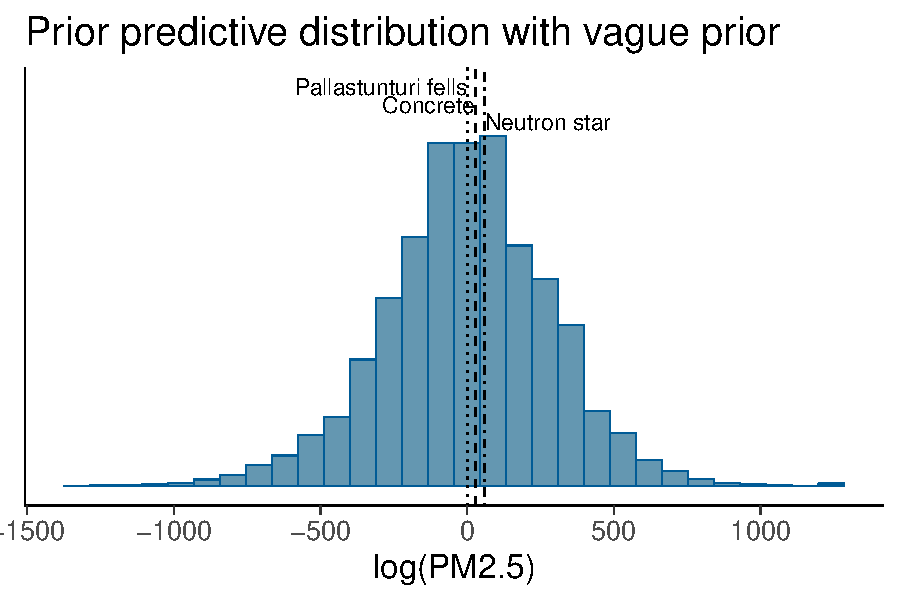
\includegraphics[width=8cm]{figs/pm25_pp1b.pdf}}
    \only<3>{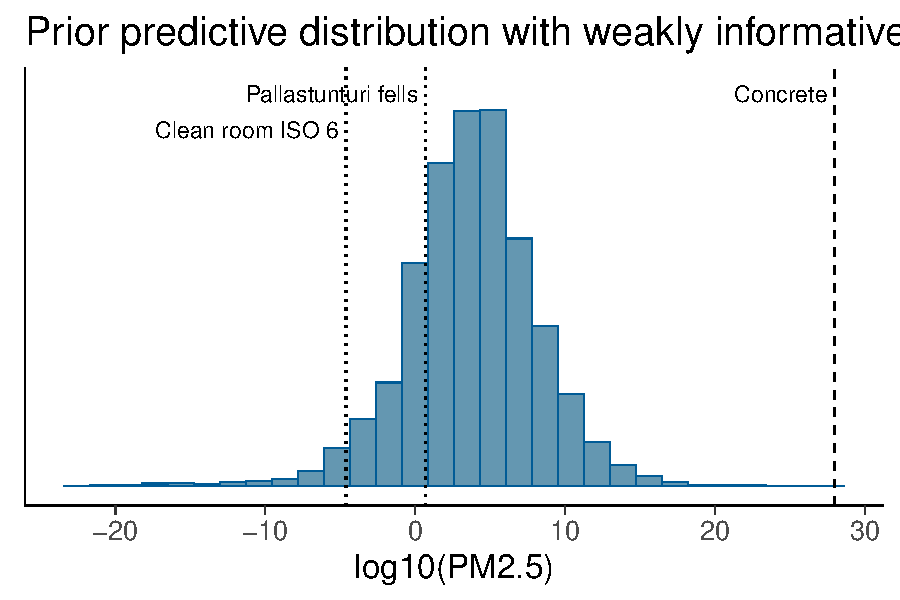
\includegraphics[width=8cm]{figs/pm25_pp2.pdf}}
\end{center}
\end{frame}

\begin{frame}

\frametitle{Example: Marginal predictive distributions}

\begin{figure}
\centering
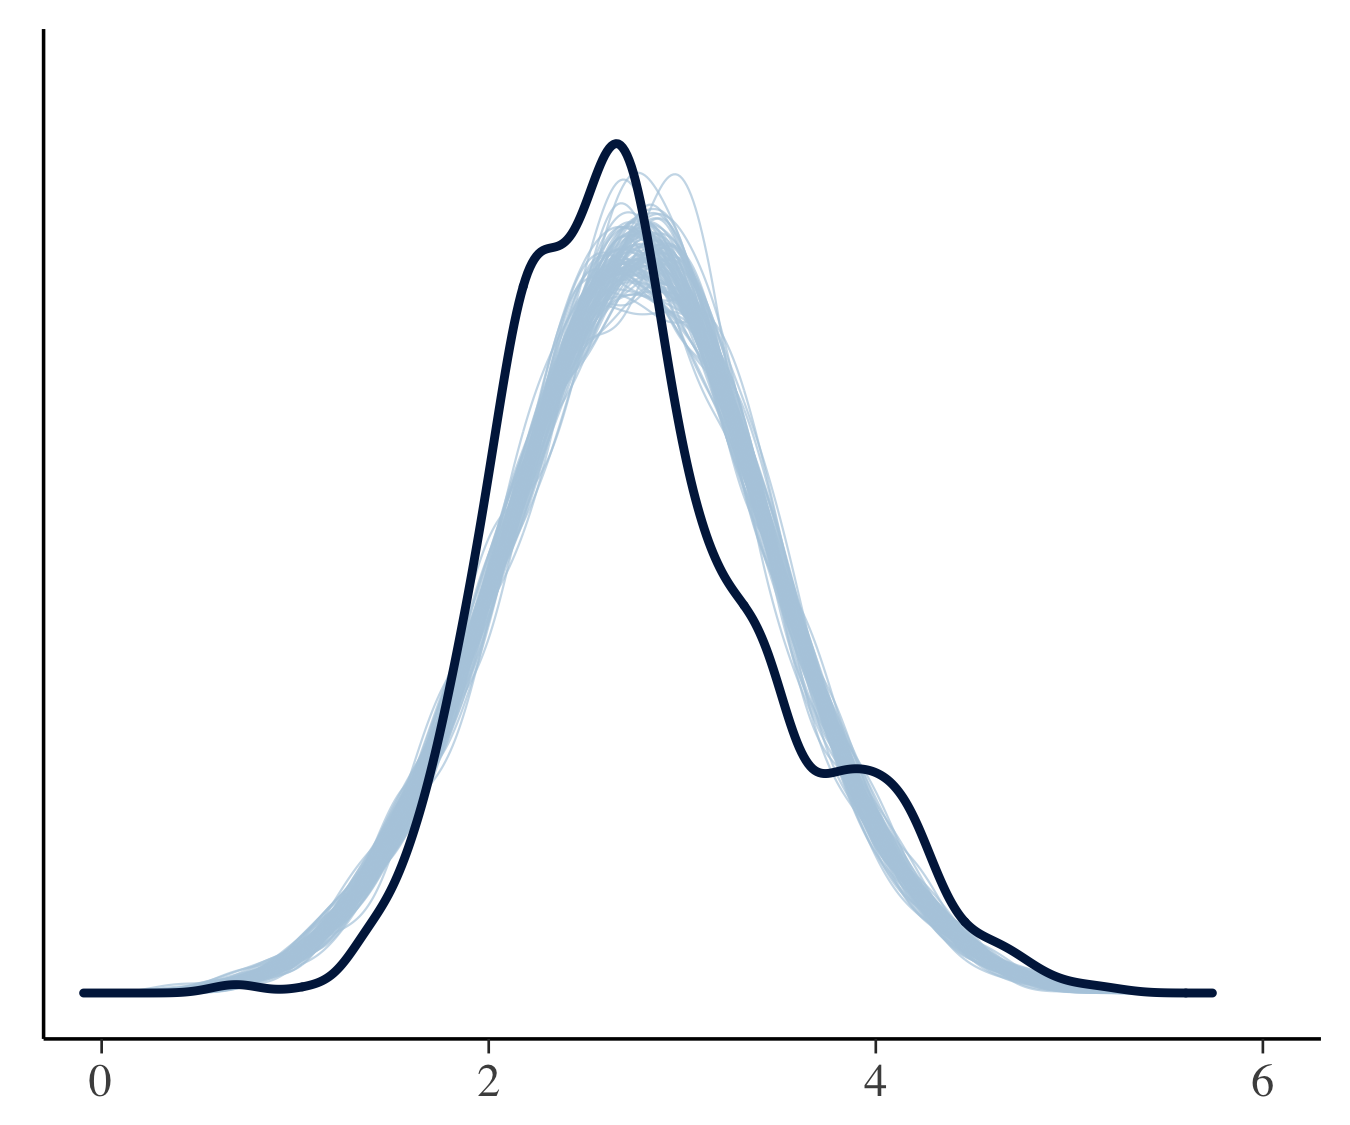
\includegraphics[width=0.9\textwidth]{figs/ppc_dens1.png}
\caption{Model 1}
\end{figure}

\end{frame}

\begin{frame}
\frametitle{Example: Marginal predictive distributions}

\begin{figure}
\centering
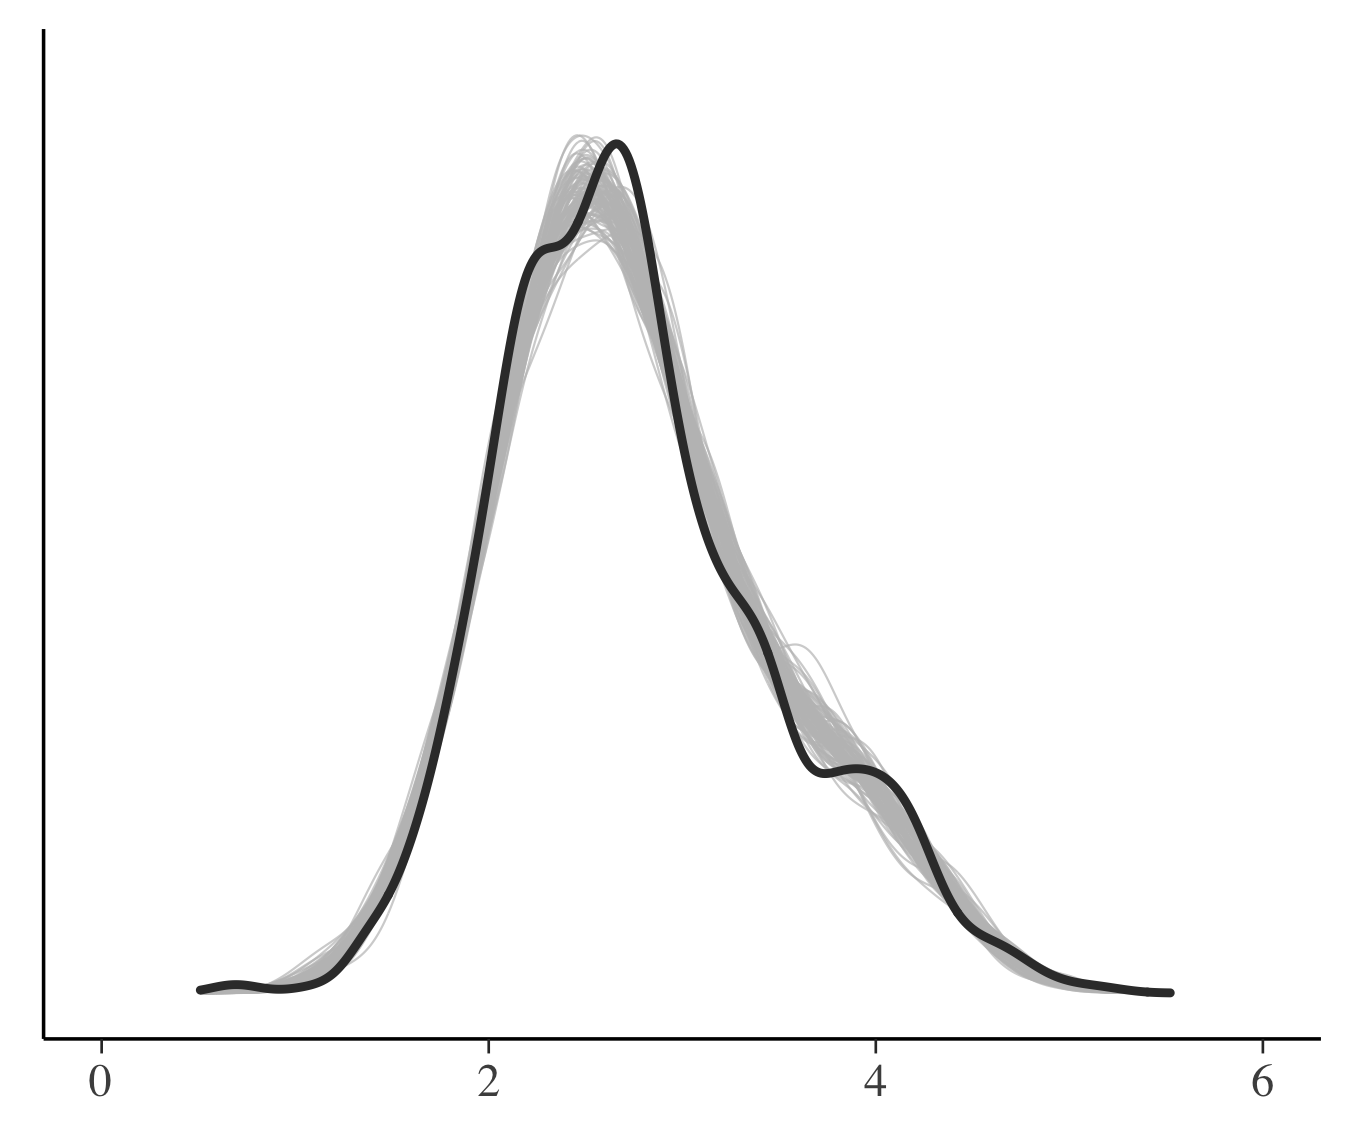
\includegraphics[width=0.9\textwidth]{figs/ppc_dens2.png}
\caption{Model 2}
\end{figure}

\end{frame}

\begin{frame}
\frametitle{Example: Marginal predictive distributions}

\begin{figure}
\centering
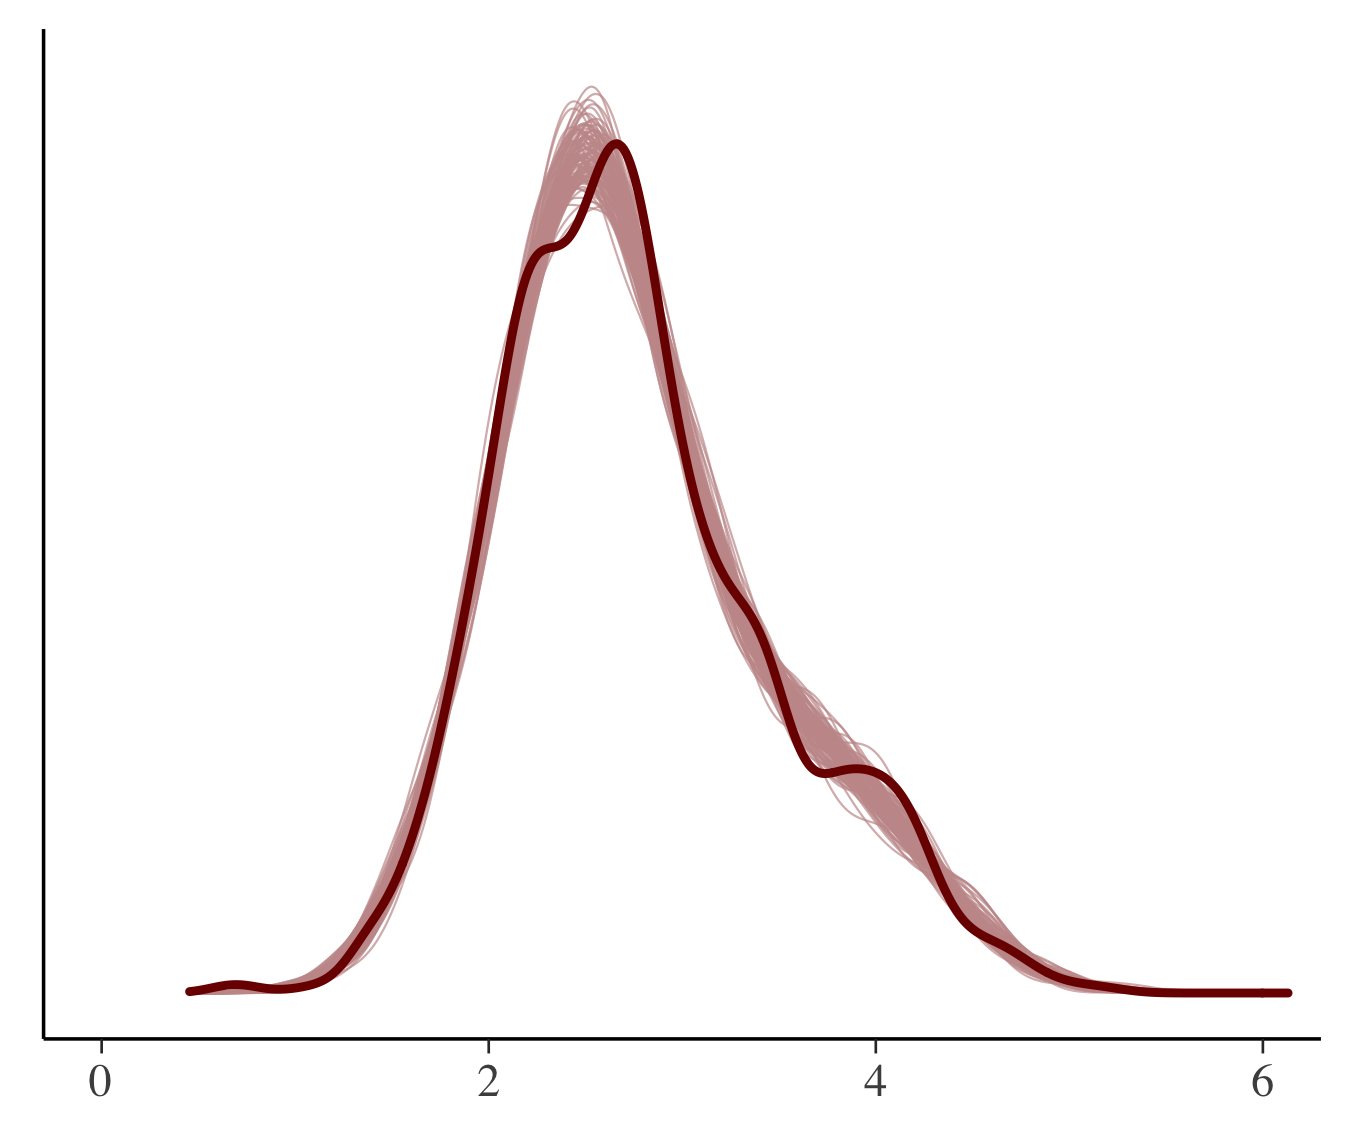
\includegraphics[width=0.9\textwidth]{figs/ppc_dens3.png}
\caption{Model 3}
\end{figure}

\end{frame}


\begin{frame}
\frametitle{Example: Test statistic (skewness)}

\begin{figure}
\centering
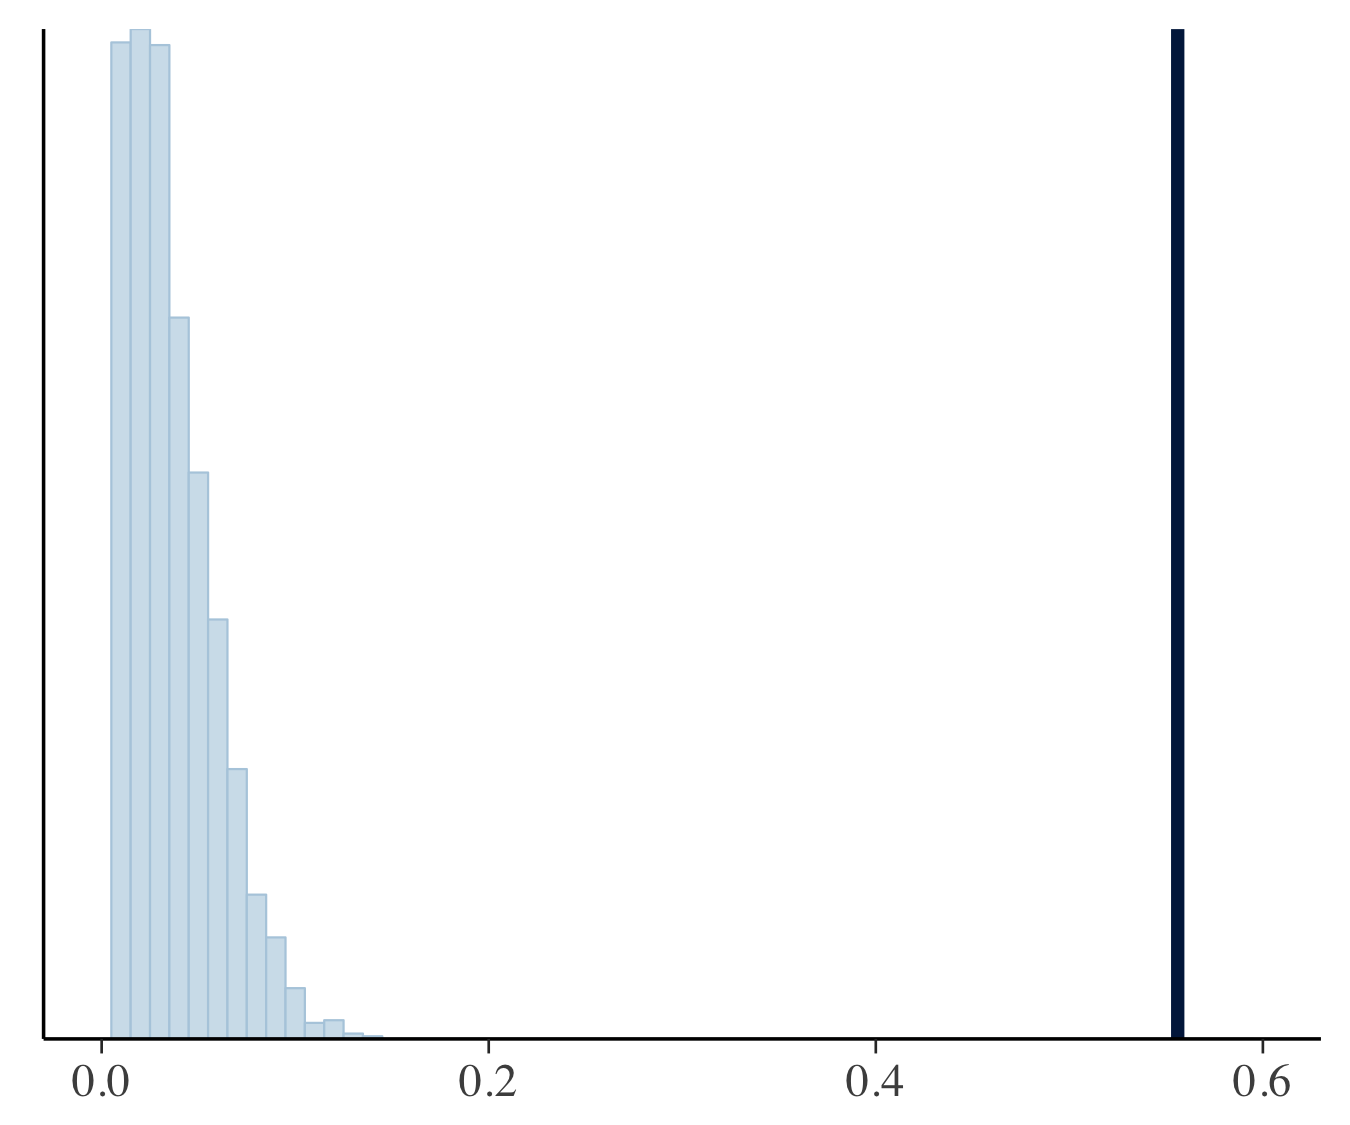
\includegraphics[width=0.9\textwidth]{figs/ppc_skew1.png}
\caption{Model 1}
\end{figure}

\end{frame}

\begin{frame}
\frametitle{Example: Test statistic (skewness)}

\begin{figure}
\centering
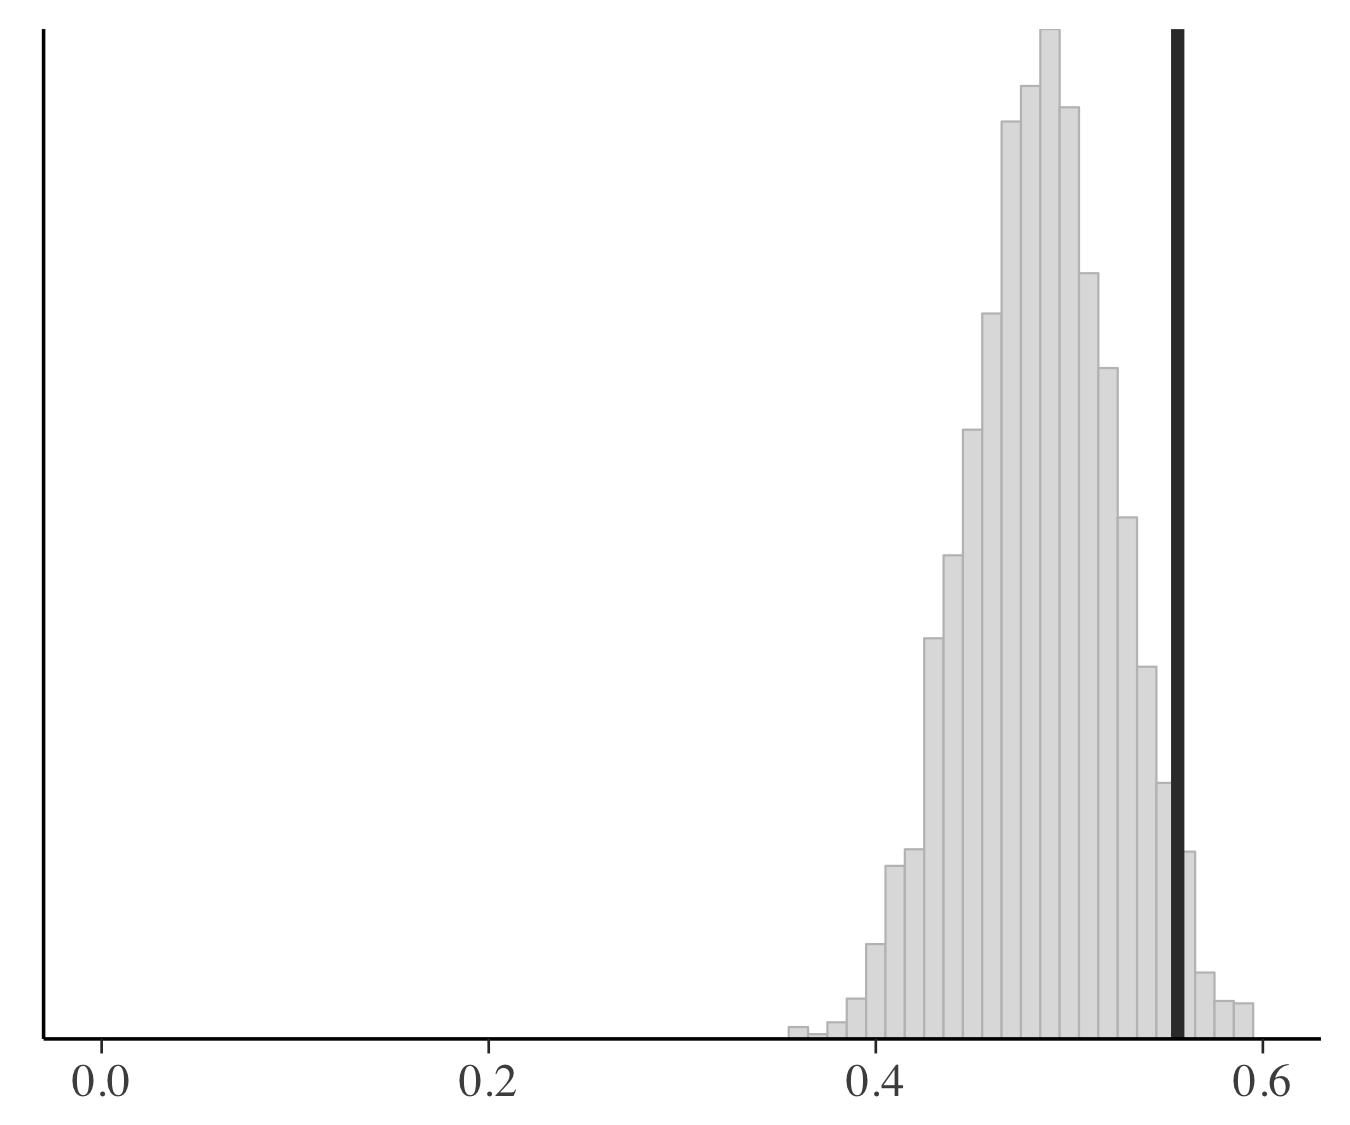
\includegraphics[width=0.9\textwidth]{figs/ppc_skew2.png}
\caption{Model 2}
\end{figure}


\end{frame}

\begin{frame}
\frametitle{Example: Test statistic (skewness)}

\begin{figure}
\centering
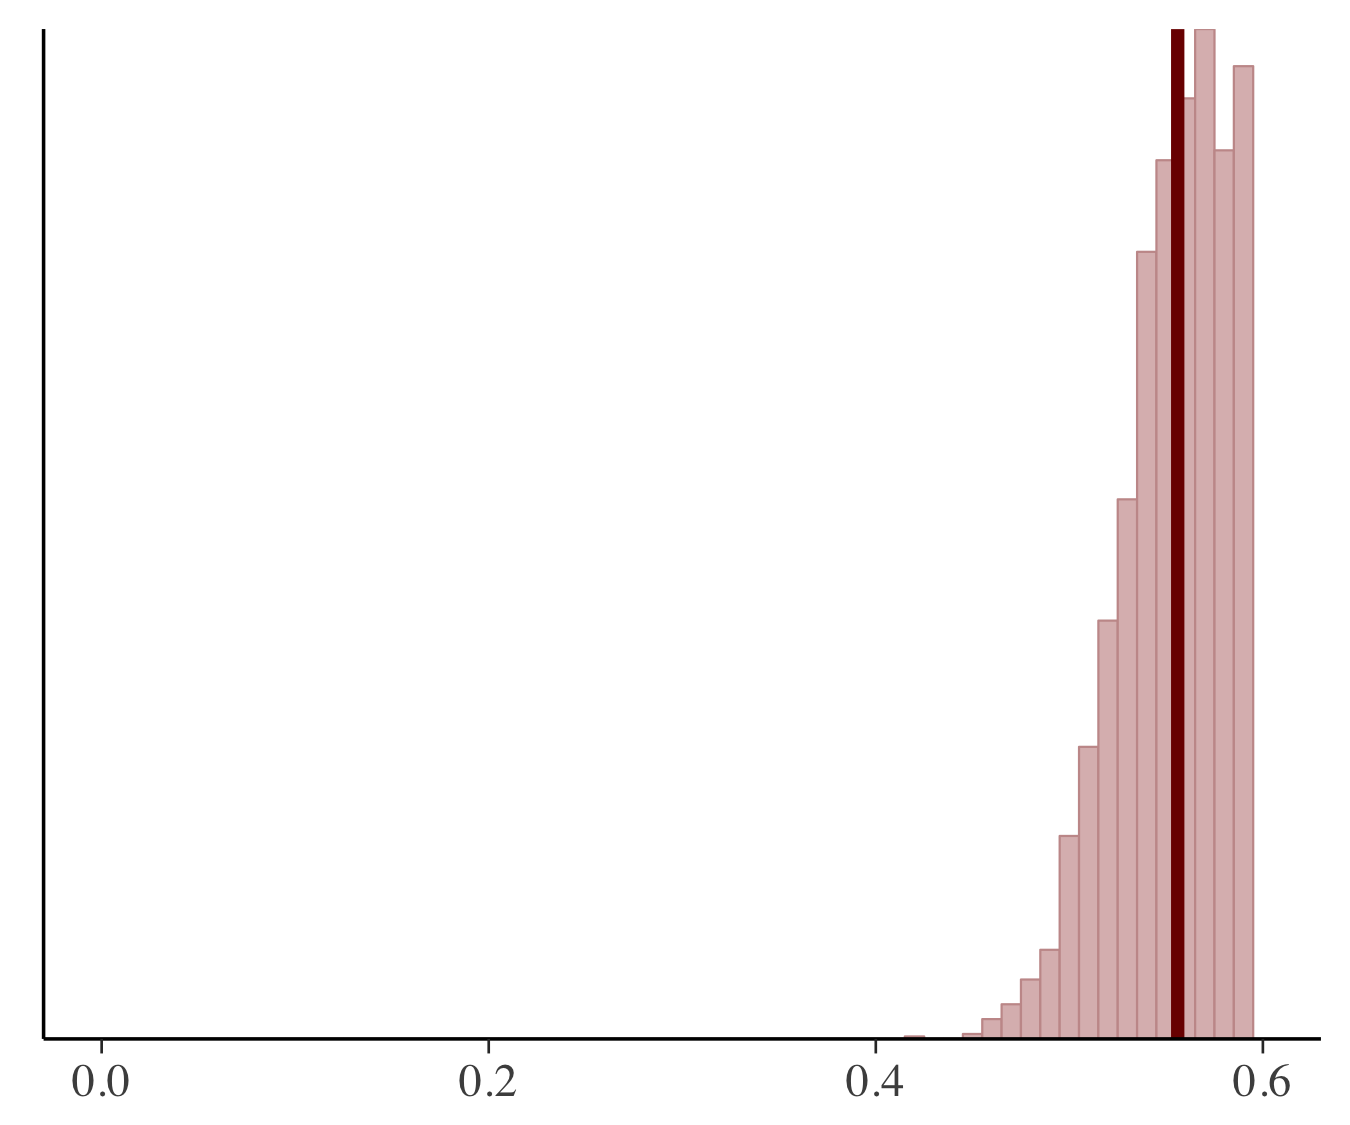
\includegraphics[width=0.9\textwidth]{figs/ppc_skew3.png}
\caption{Model 3}
\end{figure}

\end{frame}

%%%%%%%%%%%%%%%%%%%%%%%%%%%%%%%%%%%%%%%%%%%%%%%%%%%%%%%%%%%%%%%%%%


\end{document}
